\documentclass[notes=hide]{beamer}
\usepackage[ngerman]{babel} % The dictionary for hyphenation
\usepackage[utf8]{inputenc} % input-encoding
\usepackage[T1]{fontenc}    % Schriftfamilie T1 ermöglicht Trennung und
                            % Suche von Wörtern mit Umlauten.                            
\usepackage{subfig}
\usepackage{graphicx}
\usetheme{tnt}
\usepackage{subfig}

\usepackage{amsmath}
\usepackage{tabularx}
\usepackage{multirow}

\title{Lossless coding of excitation patterns in Cochlear Implants}
\author[Yan Mu, B.Eng.]{\textbf{Yan Mu}}
 \email{muyan@tnt.uni-hannover.de}
\subtitle{Konzeptvortrag Masterarbeit}
\institute{Institut für Informationsverarbeitung\\ Leibniz Universität Hannover}
\date{28.09.2018}




\begin{document}

%\maketitle

\newpage
\section{Overview}
\begin{frame}
	
   \begin{block}{Content}
   	\begin{itemize}	
		\item [•] Cochlear Implant(CI)
		\item [•] Audio signal processing(ACE)
		\item [•] Theoretical principles(entropy,Markov source,etc.)
		\item [•] Lossless coding(Huffman code,PPM,RNN)
		\item [•] Future work and Timeline
   	\end{itemize}
   \end{block}
\end{frame}   
		

\newpage
\section{Cochlear Implant(CI)}
\begin{frame}


   \begin{block}{Cochlear Implant(CI)}
   	\begin{itemize}
   		\item [•] Surgically implanted neuroprosthetic device 
   		\item [•] Microphones,sound processor and electronics(outside)
		\item [•] Coil to receive signals, electronics and electrodes which stimulate the cochlear nerve(inside)

		
   	\end{itemize}
   \end{block}
   \begin{figure}
   	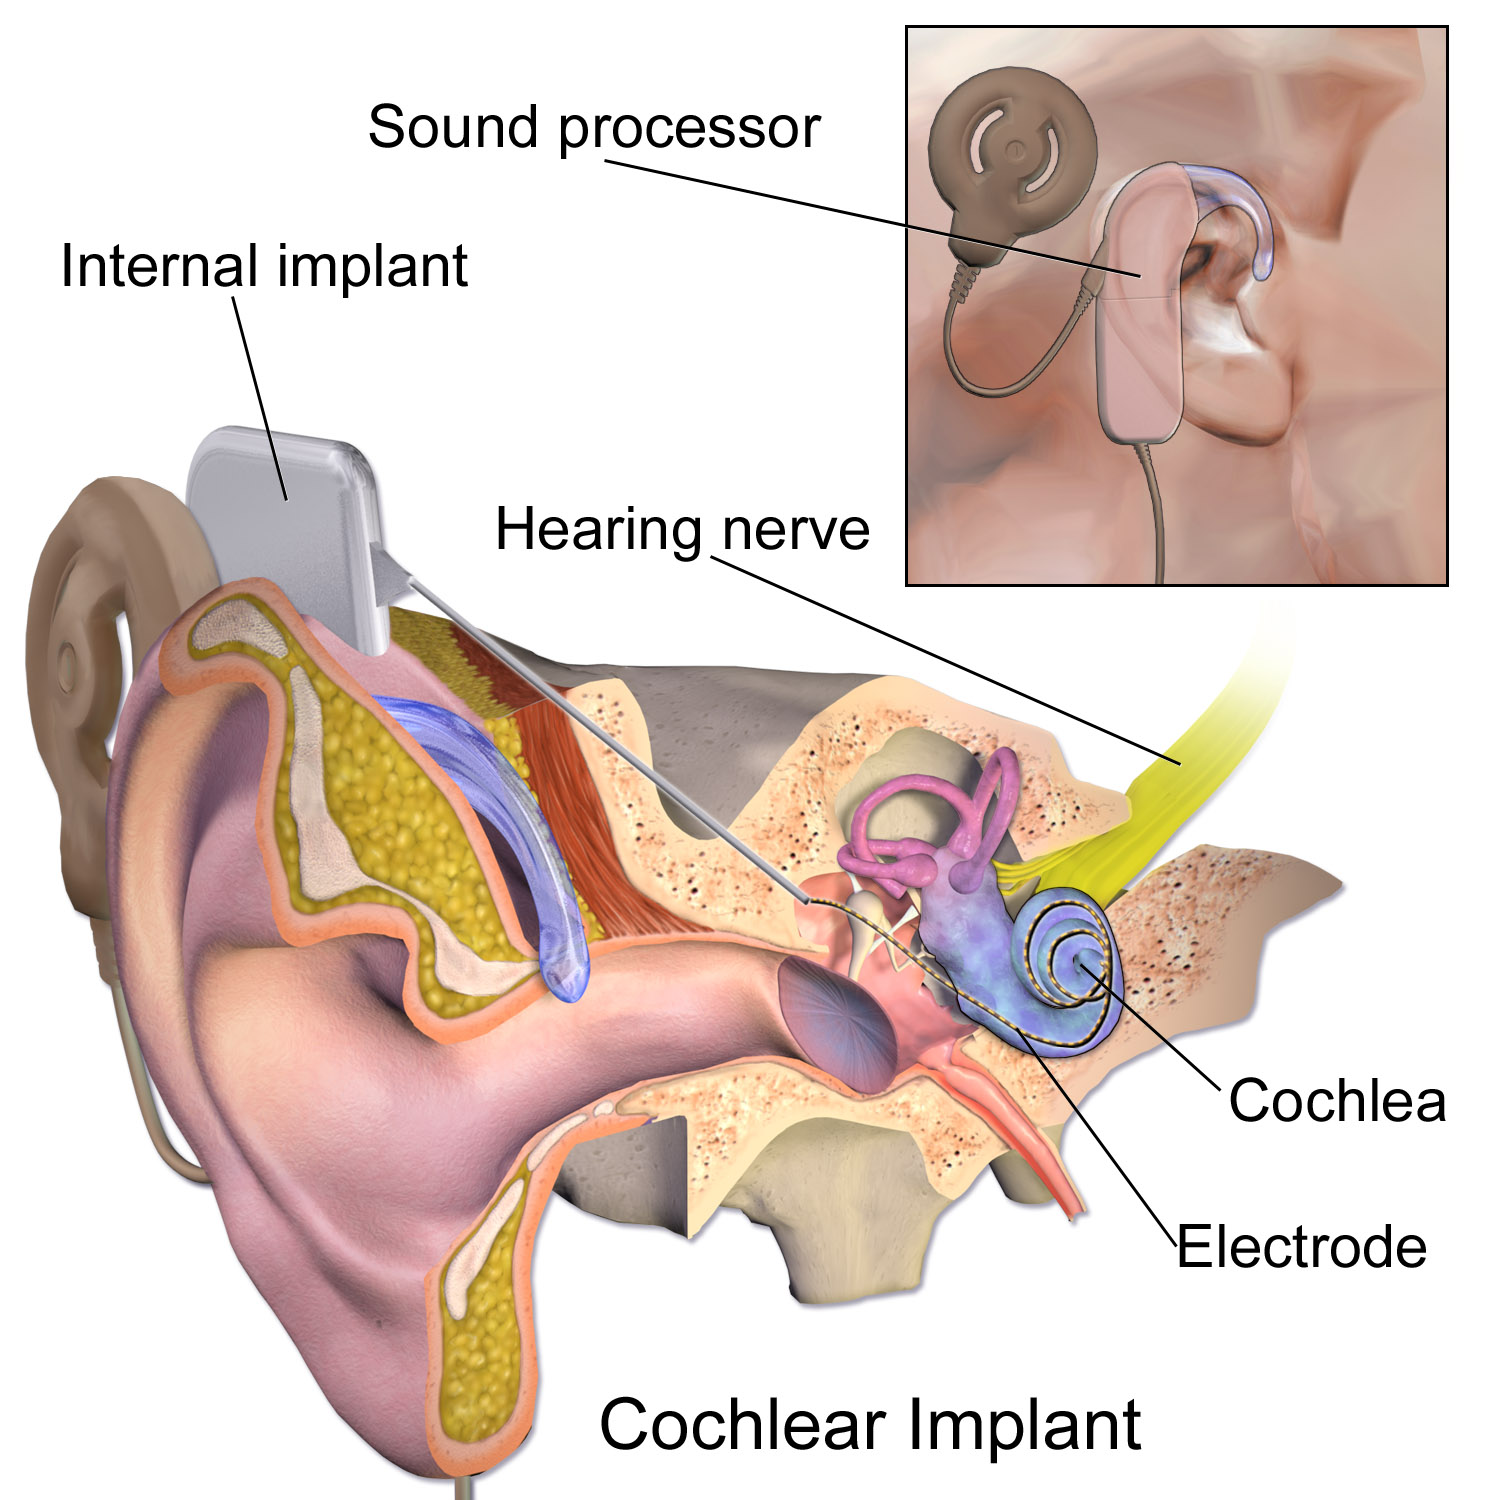
\includegraphics[scale=0.091]{Vortrag/Cochlear_implant.png}
   \end{figure}
\end{frame}


\newpage
\section{Cochlear Implant(CI)}
\begin{frame}


   \begin{block}{Problem}
   	\begin{itemize}
   		\item [•] Monaural implant, not enough in some noisy environment
   		\item [•] Binaural for improvement
		\item [•] Coding and transmission time as low as possible
		
   	\end{itemize}
   \end{block}
   \begin{figure}
   	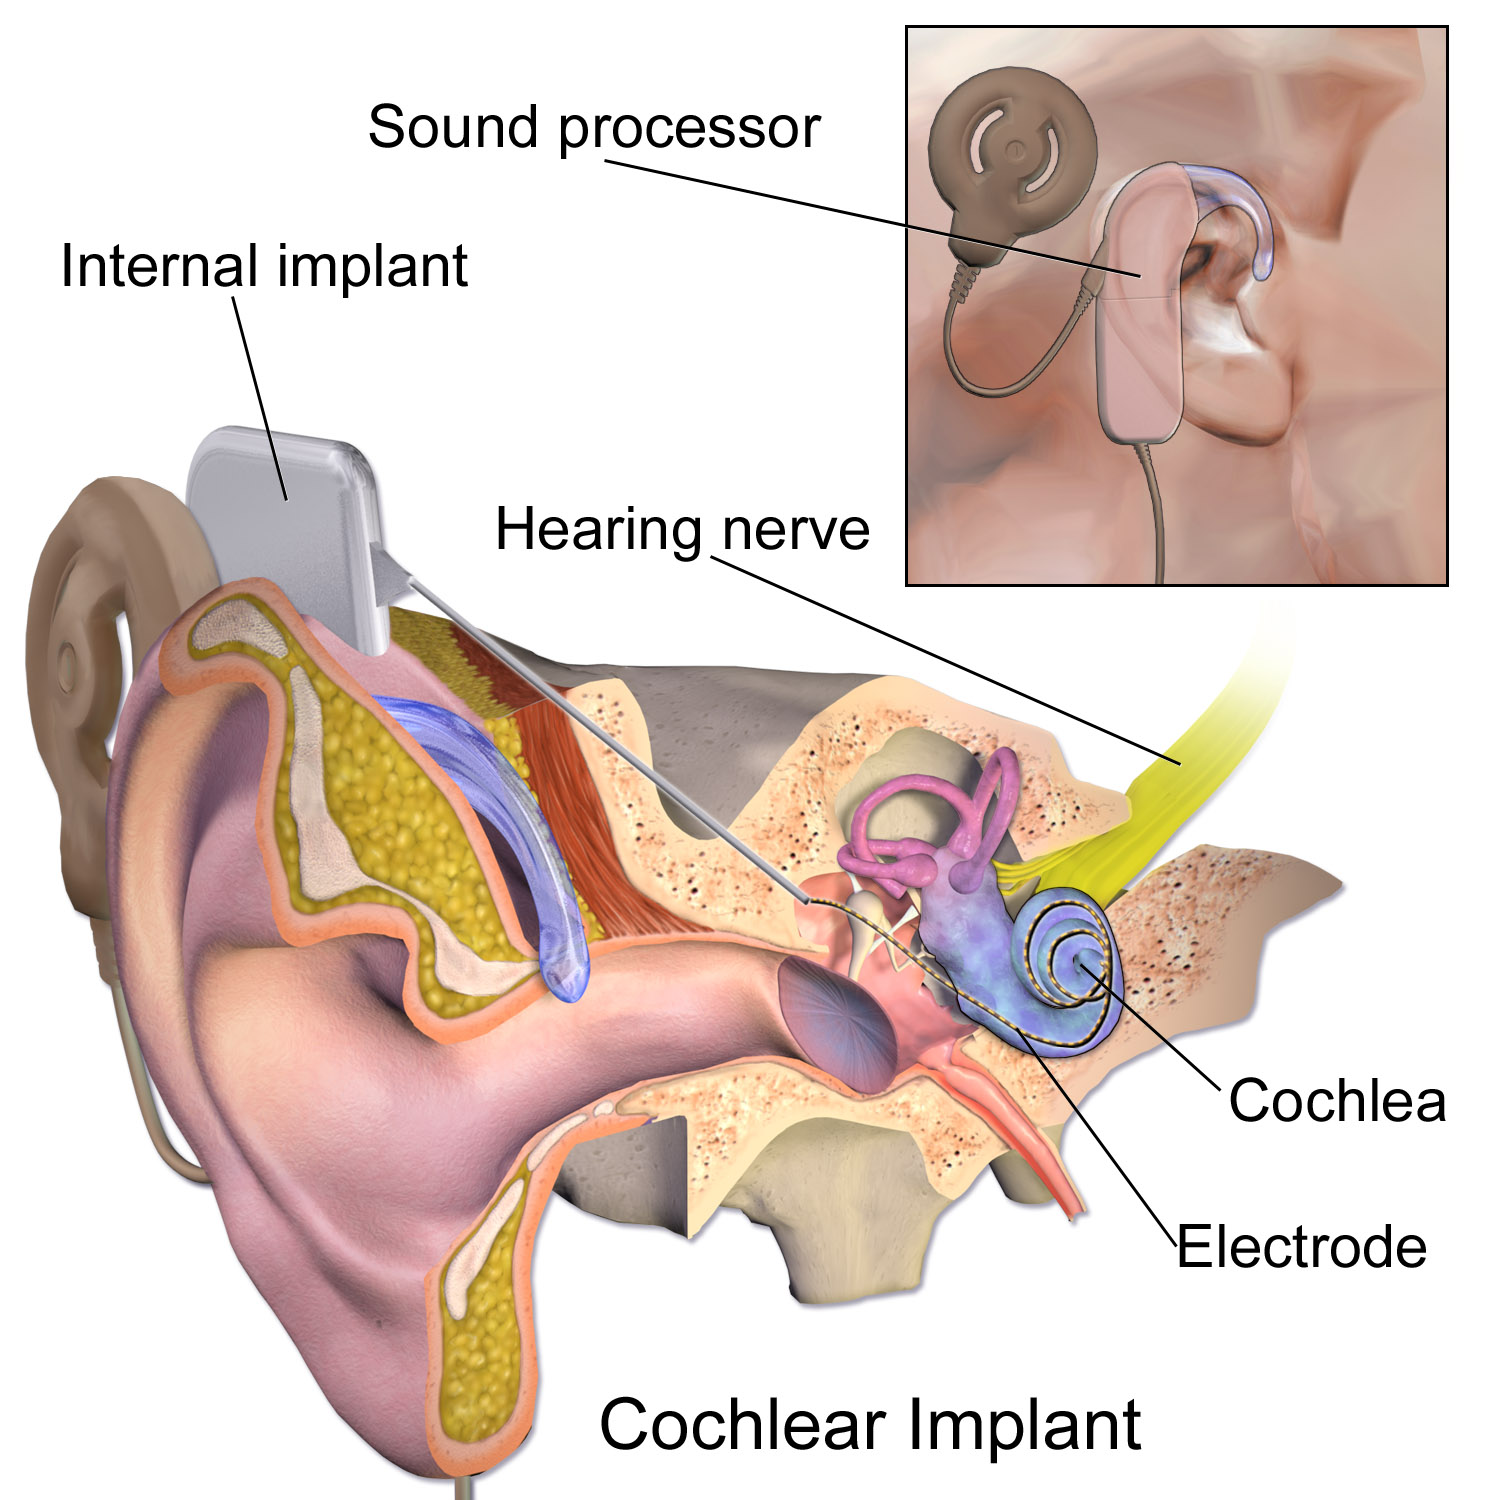
\includegraphics[scale=0.091]{Vortrag/Cochlear_implant.png}
   \end{figure}
\end{frame}


\newpage
\section{Audio signal processing}
\begin{frame}


   \begin{block}{Advanced combinational encoder(ACE)}
   	\begin{itemize}
   		\item [•] NofM-type strategy
   		\item [•] Largest amplitude envelopes are picked
		\item [•] 22 electrodes(channels)
		
   	\end{itemize}
   \end{block}
   \begin{figure}
   	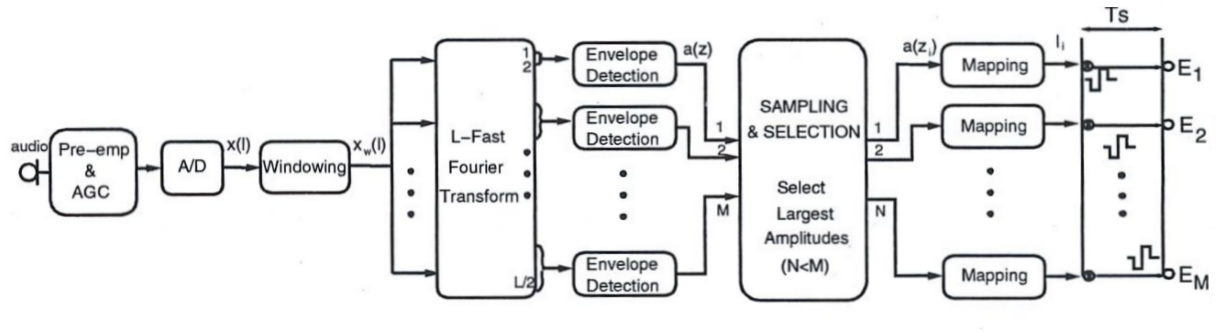
\includegraphics[scale=0.42]{Vortrag/BD_ACE.png}
   \end{figure}
\end{frame}


\newpage
\section{Audio signal processing}
\begin{frame}


   \begin{block}{Advanced combinational encoder(ACE)}
   	\begin{itemize}
		\item [•] 1 sentence which last 3 seconds 
   		\item [•] ACE generated current amplitude
   		\item [•] 22 channels, around 3000 to 8000 stimulations
   	\end{itemize}
   \end{block}
   \begin{figure}
   	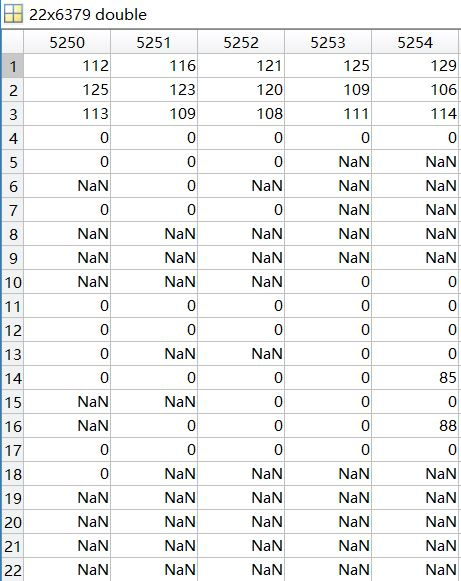
\includegraphics[scale=0.4]{Vortrag/ACE.JPG}
   \end{figure}
\end{frame}


\newpage
\section{Theoretical principles}
\begin{frame}


   \begin{block}{Entropy}
   	\begin{itemize}
   		\item [•] Lower bound of average codeword length
		\item [•] Conditional entropy for Markov source (source with memory)
		\item [•] $H(X|Y)=\sum\limits_{x\in X}^{}P(Y=y)\bullet H(X|Y=y)$
   	\end{itemize}
   \end{block}

   \begin{figure}
   	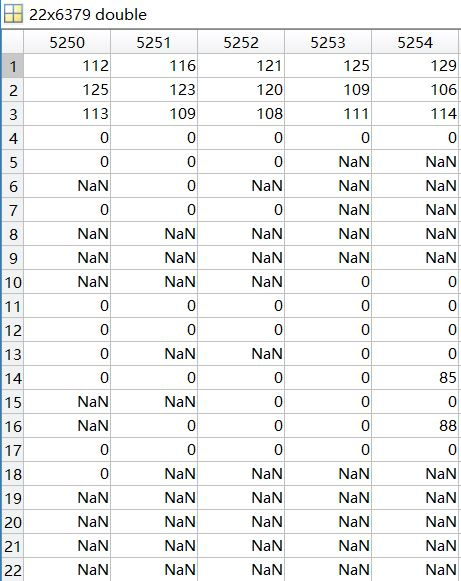
\includegraphics[scale=0.4]{Vortrag/ACE.JPG}
   \end{figure}
\end{frame}




\newpage
\section{Theoretical principles}
\begin{frame}


   \begin{block}{Conditional entropy}
   	\begin{itemize}
   		\item [•] Random selected 10 files are assembled together
   		\item [•] Unneeded zeros are deleted for clear trend
   	\end{itemize}
   \end{block}
   \begin{figure}
   	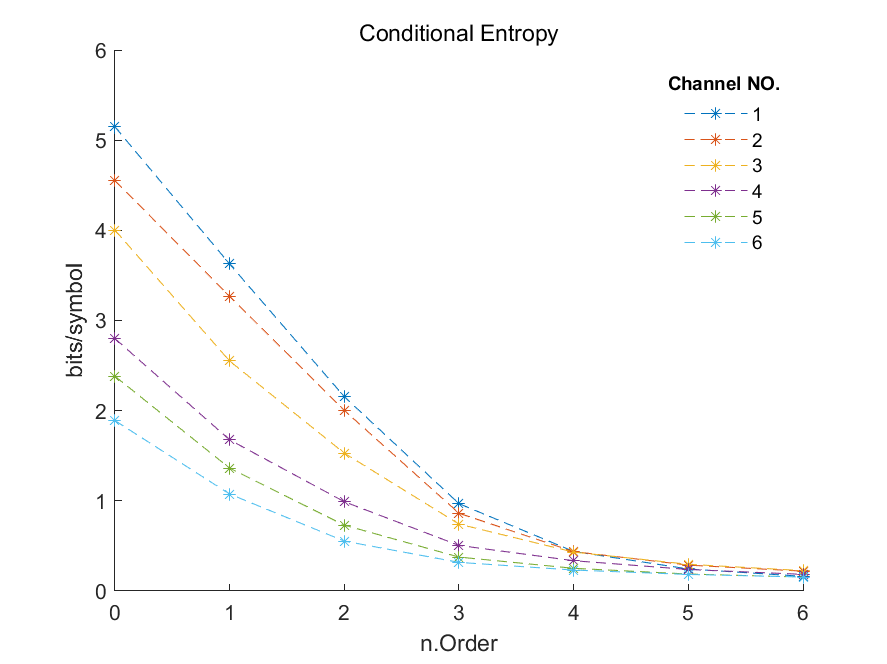
\includegraphics[scale=0.26]{Vortrag/10f6oc1to6.png}
   	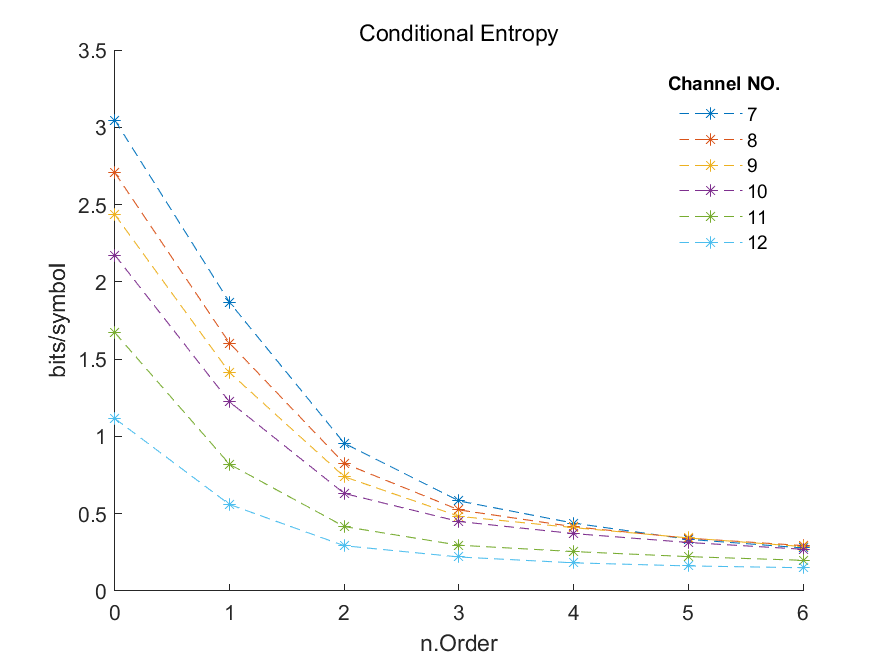
\includegraphics[scale=0.26]{Vortrag/10f6oc7to12.png}
   	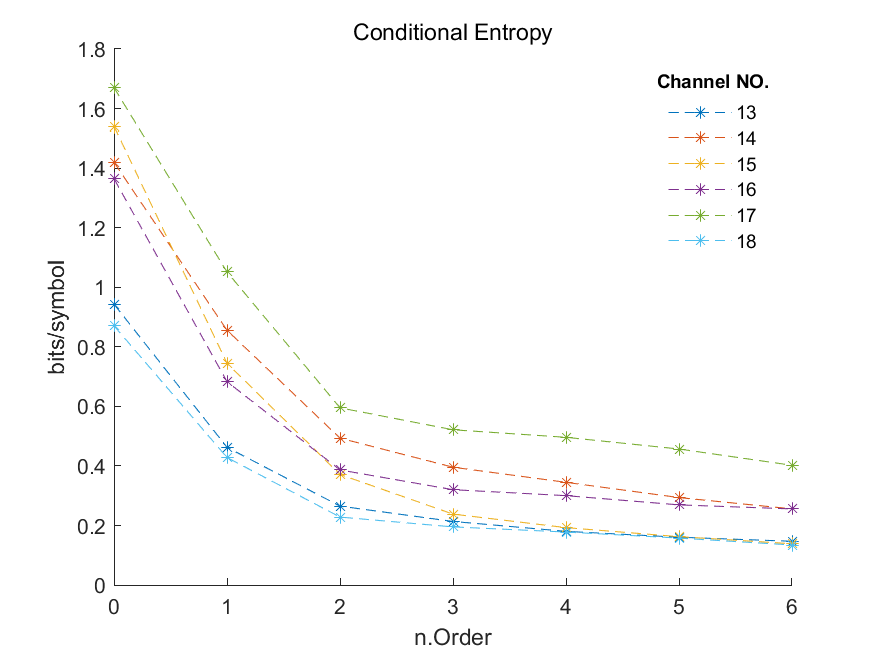
\includegraphics[scale=0.26]{Vortrag/10f6oc13to18.png}
   	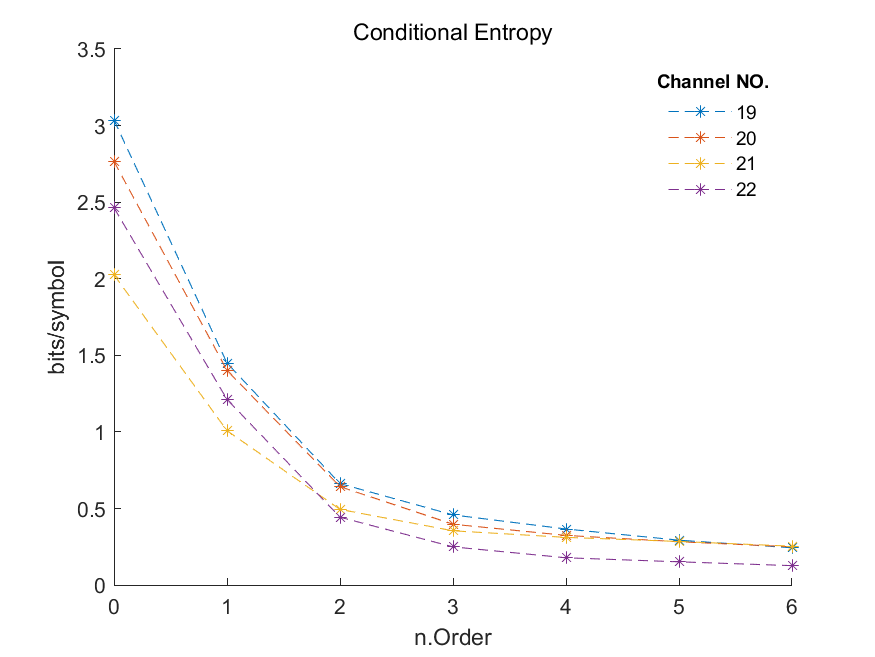
\includegraphics[scale=0.26]{Vortrag/10f6oc19to22.png}
   \end{figure}
\end{frame}


\newpage
\section{Theoretical principles}
\begin{frame}


   \begin{block}{Conditional entropy}
   	\begin{itemize}
   		\item [•] Random selected 10, 20, 50 and 100 files
   		\item [•] channel 1 to 6
   	\end{itemize}
   \end{block}
   \begin{figure}
   	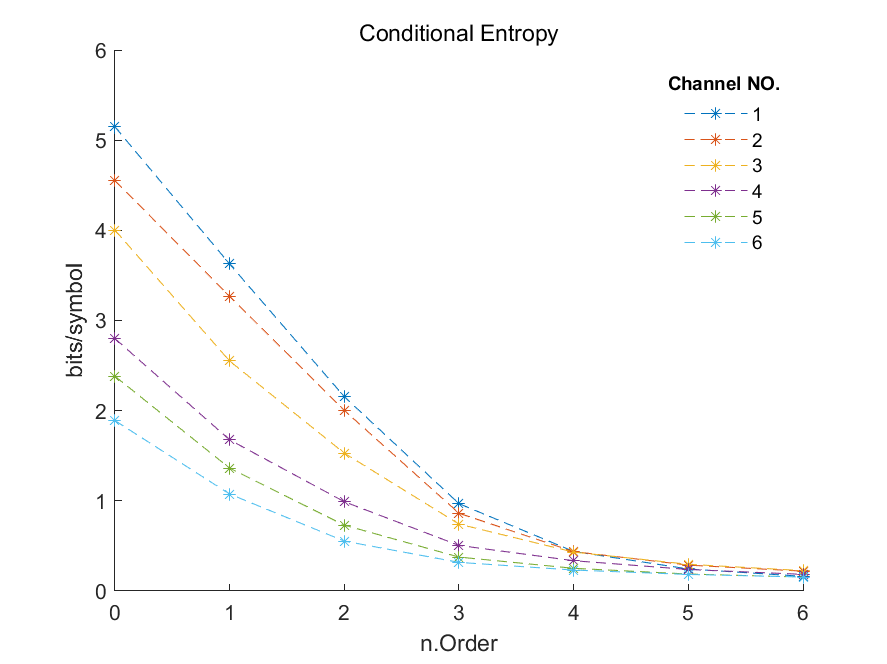
\includegraphics[scale=0.26]{Vortrag/10f6oc1to6.png}
   	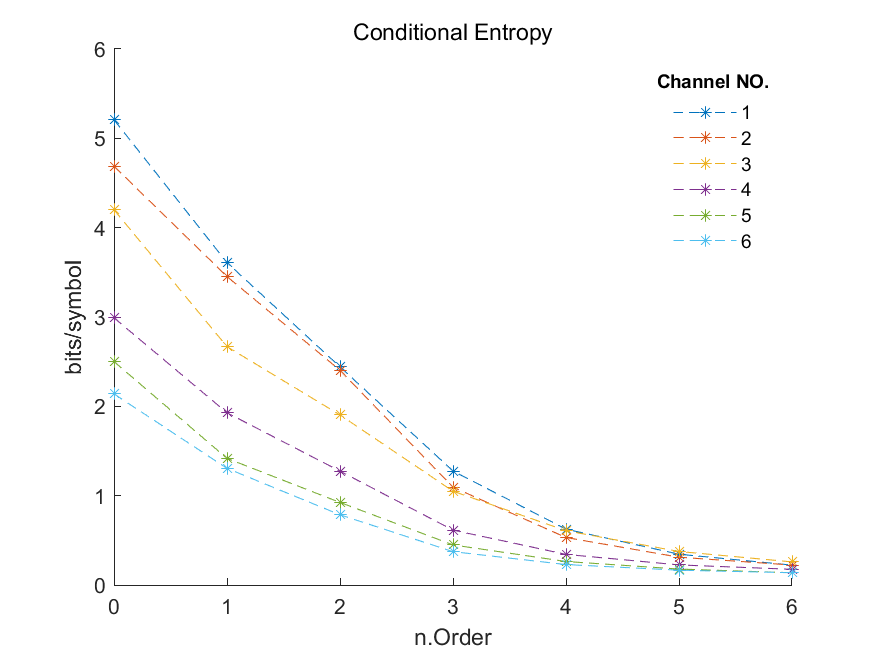
\includegraphics[scale=0.26]{Vortrag/20f6oc1to6.png}
   	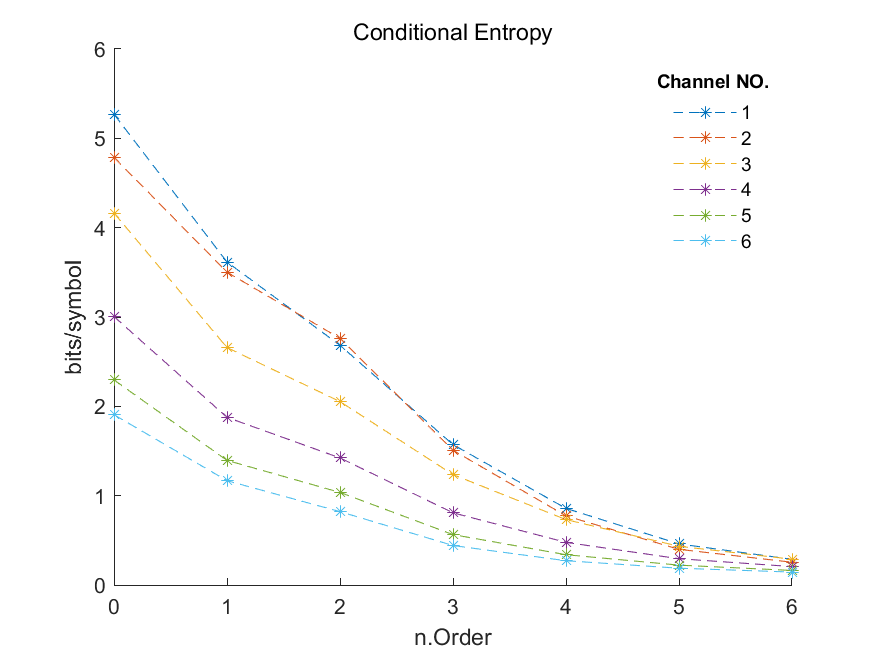
\includegraphics[scale=0.26]{Vortrag/50f6oc1to6.png}
   	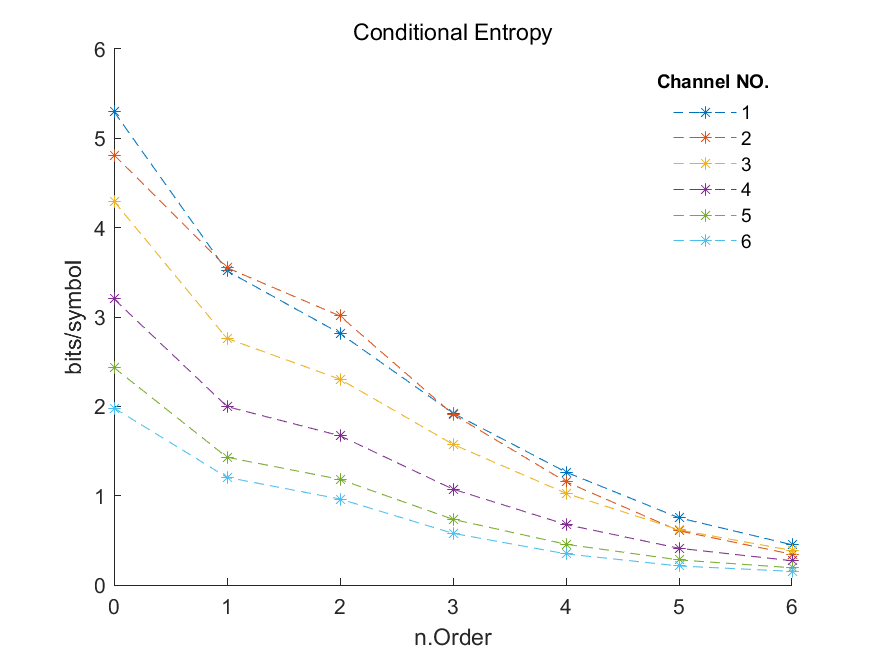
\includegraphics[scale=0.26]{Vortrag/100f6oc1to6.png}
   \end{figure}
\end{frame}


\newpage
\section{Lossless coding}
\begin{frame}


   \begin{block}{Huffman code}
   	\begin{itemize}
   		\item [•] Optimal prefix code for lossless coding
   		\item [•] $\frac{H(U_N|U_1,...,U_N-1)}{log_2 D}\leq\overline{\rm n}<\frac{H(U_N|U_1,...,U_N-1)}{log_2 D}+1$
   		\item [•] A Markov source of n order has up to $J=K^{n-1}$ different states, means $J$ different prefix codes required 
   		\item [•] For our ACE generated source, $K\approx 72$. The order 6 Huffman code requires $1.9349\times10^9$ different prefix codes
   		\item [•] Impracticable because of high computational effort
   		
   	\end{itemize}
   \end{block}
\end{frame}


\newpage
\section{Lossless coding}
\begin{frame}


   \begin{block}{Prediction by partial string matching(PPM)}
   	\begin{itemize}
   		\item [•] Very high compression rates
        \item [•] Use a set of previous symbols in the uncompressed symbol stream to predict the next symbol
   		\item [•] Particularly suitable for our Markov source data
   	\end{itemize}
   \end{block}
\end{frame}


\newpage
\section{Lossless coding}
\begin{frame}


   \begin{block}{Prediction by partial string matching(PPM)}
   	\begin{itemize}
   		\item [•] Use Markov Modelling with Partial String Matching to estimate probability
   		\item [•] Estimates escape probabilities for 'zero frequency problem'
        \item [•] Probability table is fed to arithmetic coder in order to encode data
   	\end{itemize}
   \end{block}    

\end{frame}


\newpage
\section{Lossless coding}
\begin{frame}


   \begin{block}{Prediction by partial string matching(PPM)}
   	\begin{itemize}
   		\item [•] Probability of symbol $\varphi$: $p(\varphi)=\frac{c(\varphi)}{1+C}, c(\varphi)>0$
        \item [•] Escape probability $1-\sum\limits_{\varphi\in K,c(\varphi)>0}p(\varphi)=\frac{1}{1+C}$ 
        \item [•] $p(133)=\frac{1}{12}\times\frac{1}{4}\times\frac{1}{27}\times\frac{32}{105}$
        \item [•] If current symbol is novel even to the zero order context, final escape, encoded as an 8 bit code
   	\end{itemize}
   \end{block}    
\begin{tabular}{|c|c|l l l l l l l|c|}
  \hline
  order & context & \multicolumn{7}{c|}{symbol occurrence counts} & total \\ 
  &					& 0 & 81 & 85 & 110	&112 & 121 & 133 & \\	 	
  \hline \hline
  3 & (112,116,121) & 9 & 2  & & & & & & 11 \\
  \hline
  2 & (112,116)		& 10& 2  & 3 & & & & & 15 \\
  \hline
  1 & (116)			& 15& 6  & 18 & 25 & 1 & & & 65 \\
  \hline
  0 & empty 		& 30& 15 & 41 & 68 & 24 & 72 & 32 &282\\
  \hline 
\end{tabular} 
\end{frame}


\newpage
\section{Lossless coding}
\begin{frame}


   \begin{block}{Prediction by partial string matching(PPM)}
   	\begin{itemize}
   		\item [•] Individual encoding for every channel 
   		\item [•] Pack all 22 channels for transmission		
   	\end{itemize}
   \end{block}
   \begin{figure}
   	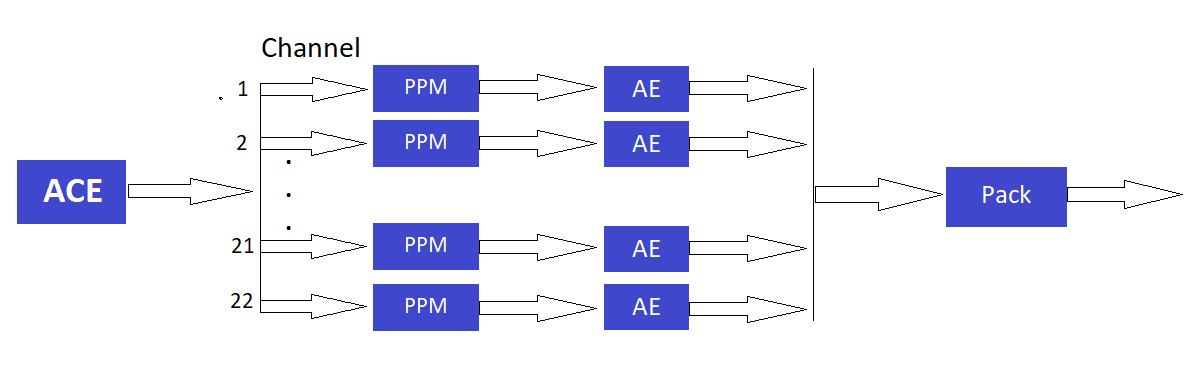
\includegraphics[scale=0.48]{Vortrag/PPM.jpg}
   \end{figure}
\end{frame}



\newpage
\section{Lossless coding}
\begin{frame}


   \begin{block}{Lossless Compression using Recurrent Neural Networks}
   	\begin{itemize}
   		\item [•] RNN(LSTM/GRU) based models are good at capturing long term dependencies 
        \item [•] RNN(LSTM/GRU) can predict the next symbol very well
		\item [•] RNN(LSTM/GRU) is highly potential for lossless compression (according to existing research, DeepZip)
   	\end{itemize}
   \end{block}
\end{frame}

\newpage
\section{Lossless coding}
\begin{frame}


   \begin{block}{Lossless Compression using Recurrent Neural Networks}
   	\begin{itemize}
   		\item [•] Similar structure to PPM
        \item [•] Both consist of probability estimator and arithmetic encoder
		\item [•] DeepZip estimates conditional entropy distribution through RNN 
   	\end{itemize}
   \end{block}
   \begin{figure}
   	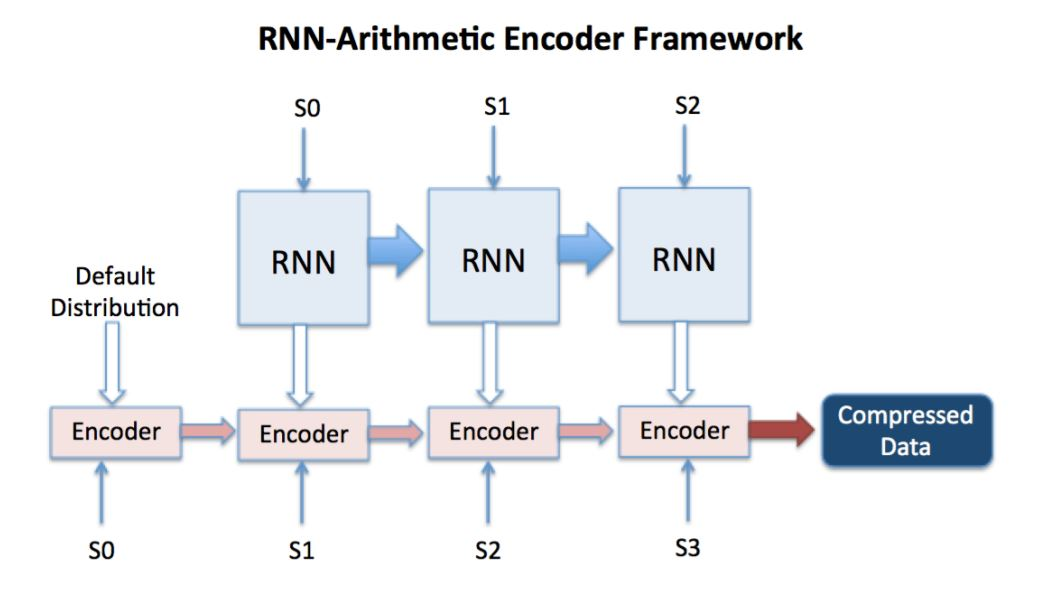
\includegraphics[scale=0.4]{Vortrag/DeepZip.jpg}
   \end{figure}
\end{frame}


\newpage
\section{Future work and Timeline}
\begin{frame}


   \begin{block}{Timeline}
   	\begin{itemize}
   		\item [•] In 3 weeks test PPM for our project 
        \item [•] In 6 weeks test DeepZip for our project
		\item [•] Compare 2 different coding methods 
		\item [-] Computational effort(code and decode time)
		\item [-] Storage memory demands
		\item [-] etc.
   	\end{itemize}
   \end{block}
\end{frame}



\end{document}